\chapter{Project Management}
\label{project management}

\section{The Group}
The group formed out of the desire to work together based on varying levels of previous experience working together, rather than out of a desire to work on a specific project as was the case with other groups.
The group quickly decided to take advantage of the new iLab at Warwick University and chose to make use of the Microsoft Kinect.
Initial ideas revolved around object modelling and sharing, but due to the low resolution of the Kinect, these early ideas were abandoned.
After discussions with the project supervisor, the group chose to tackle the problem proposed by \todo{the italians}.\\

\begin{figure}[h]
\begin{center}
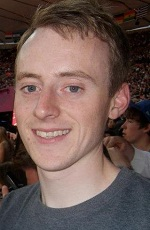
\includegraphics[scale=0.5]{./pm/bernard}
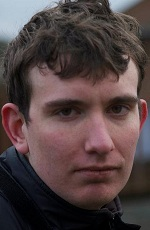
\includegraphics[scale=0.5]{./pm/greg}

\includegraphics[scale=0.5]{./pm/nathan}
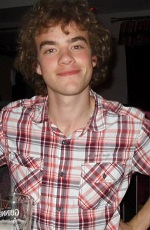
\includegraphics[scale=0.5]{./pm/robin}

\includegraphics[scale=0.5]{./pm/stef} 
\end{center}
\caption{The group from left to right: Bernard, Greg, Nathan, Robin and Paps.}
\label{fig:the group}
\end{figure}

\section{Group Behaviour}

\subsection{Weekly Meetings}
The group organised weekly meeting, in which the activities from the last week would come under review. This review process is described more in Section \ref{pm:peer review process}.
As well as looking at progress from the last week, tasks for the upcoming week would be discussed and assigned to team members.\\

\subsection{Group Coding Sessions}
Often, the group would congregate around the Kinect in CS0.01 within the Computer Science Department at Warwick to work on the project. The group would use these occasions to provide fresh insight into individual problems.\\

\subsection{Peer Review Process}
\label{pm:peer review process}


\subsection{Centralised Code Repository}
The group made use of a Git repository to manage source code, which whilst it had a steep learning curve, has avoided any version control issues.

\subsection{Self organising Sub Committees}

\subsection{Clear Task Responsibility}

\subsection{Morale}
\label{morale}
In order to maintain a high group morale, many "memes" were created out of the group to lift spirits and keep humour present after particularly tense group meetings. A selection is reproduced in Figures \ref{fig:we're meeting now?} through to \ref{fig:sexy sexton}

\begin{figure}[h]
\begin{center}
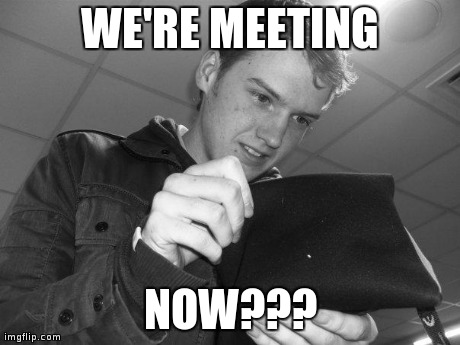
\includegraphics[scale=0.4]{./design/nathan} 
\end{center}
\caption{We're meeting now?}
\label{fig:we're meeting now?}
\end{figure} 

\begin{figure}[h]
\begin{center}
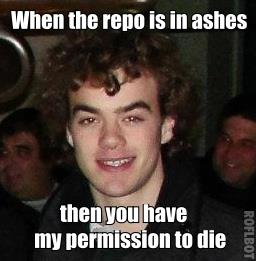
\includegraphics[scale=0.4]{./design/banerobin}
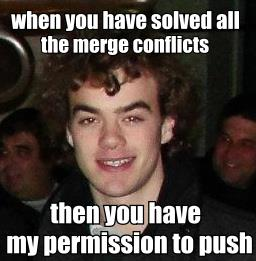
\includegraphics[scale=0.4]{./design/banerobin2}  
\end{center}
\caption{Good guy / Scum bag Robin}
\label{fig:scum bag robin}
\end{figure}

\begin{figure}[h]
\begin{center}
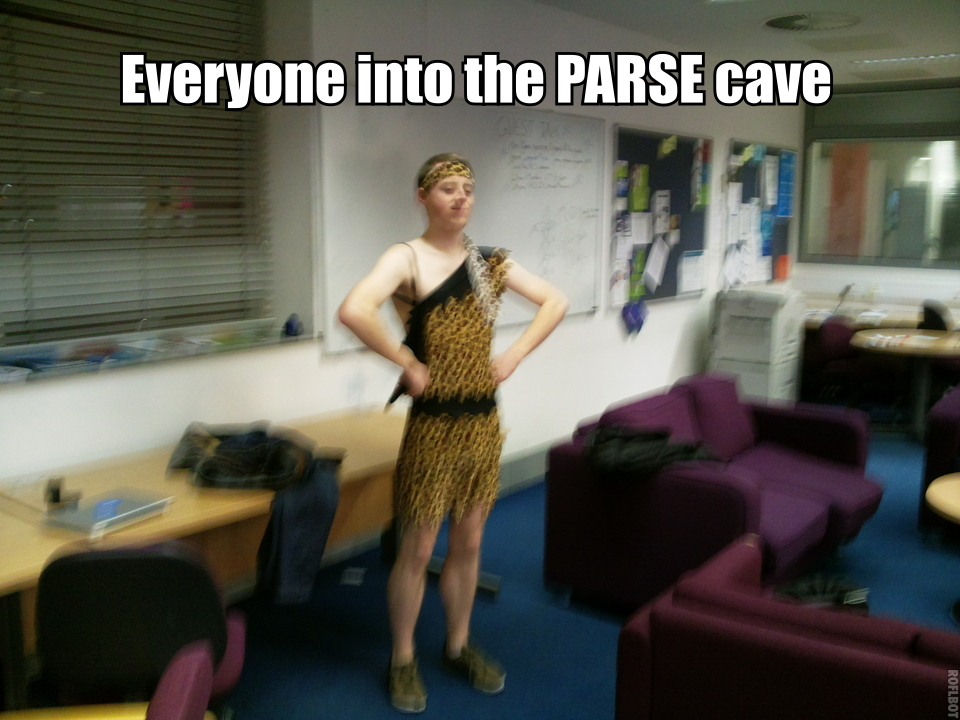
\includegraphics[scale=0.4]{./design/PARSECave} 
\end{center}
\caption{Sexy Sexton}
\label{fig:sexy sexton}
\end{figure} 
